\documentclass[tikz,border=8pt]{standalone}
\usepackage[T1]{fontenc}
\usepackage{helvet}
\renewcommand{\familydefault}{\sfdefault}
\usetikzlibrary{arrows.meta,positioning,shapes.geometric,fit,backgrounds}

\definecolor{ink}{HTML}{222222}
\definecolor{line}{HTML}{6B7280}
\definecolor{soft}{HTML}{F8FAFC}
\definecolor{accent}{HTML}{2563EB}
\definecolor{mint}{HTML}{059669}
\definecolor{amber}{HTML}{D97706}
\definecolor{rose}{HTML}{DC2626}

\tikzset{
  umlpanel/.style={draw=black!55, fill=white, line width=0.45pt},
  title/.style={font=\bfseries\small, text=ink},
  activity/.style={rounded corners=2pt, draw=line, fill=soft, align=center,
    text width=2.45cm, minimum height=7mm, inner sep=2.5pt, font=\scriptsize},
  activitywide/.style={rounded corners=2pt, draw=line, fill=soft, align=center,
    text width=3.0cm, minimum height=7mm, inner sep=2.5pt, font=\scriptsize},
  decision/.style={diamond, draw=line, fill=white, aspect=2.0, align=center,
    inner sep=1pt, text width=1.55cm, font=\scriptsize},
  start/.style={circle, fill=ink, minimum size=4pt, inner sep=0pt},
  stop/.style={circle, draw=ink, line width=0.7pt, minimum size=6pt, inner sep=0pt,
    path picture={\fill[ink] (path picture bounding box.center) circle (2pt);}},
  flow/.style={-{Latex[length=2mm,width=1.4mm]}, draw=ink!70, line width=0.55pt},
  note/.style={font=\tiny, text=black!55, align=center},
}

\newcommand{\panelgrid}[2]{%
  \begin{scope}[on background layer]
    \node[umlpanel, fit=#1, inner sep=5mm] (#2box) {};
    \draw[step=4mm, black!6, line width=0.2pt] (#2box.south west) grid (#2box.north east);
  \end{scope}
}

\begin{document}
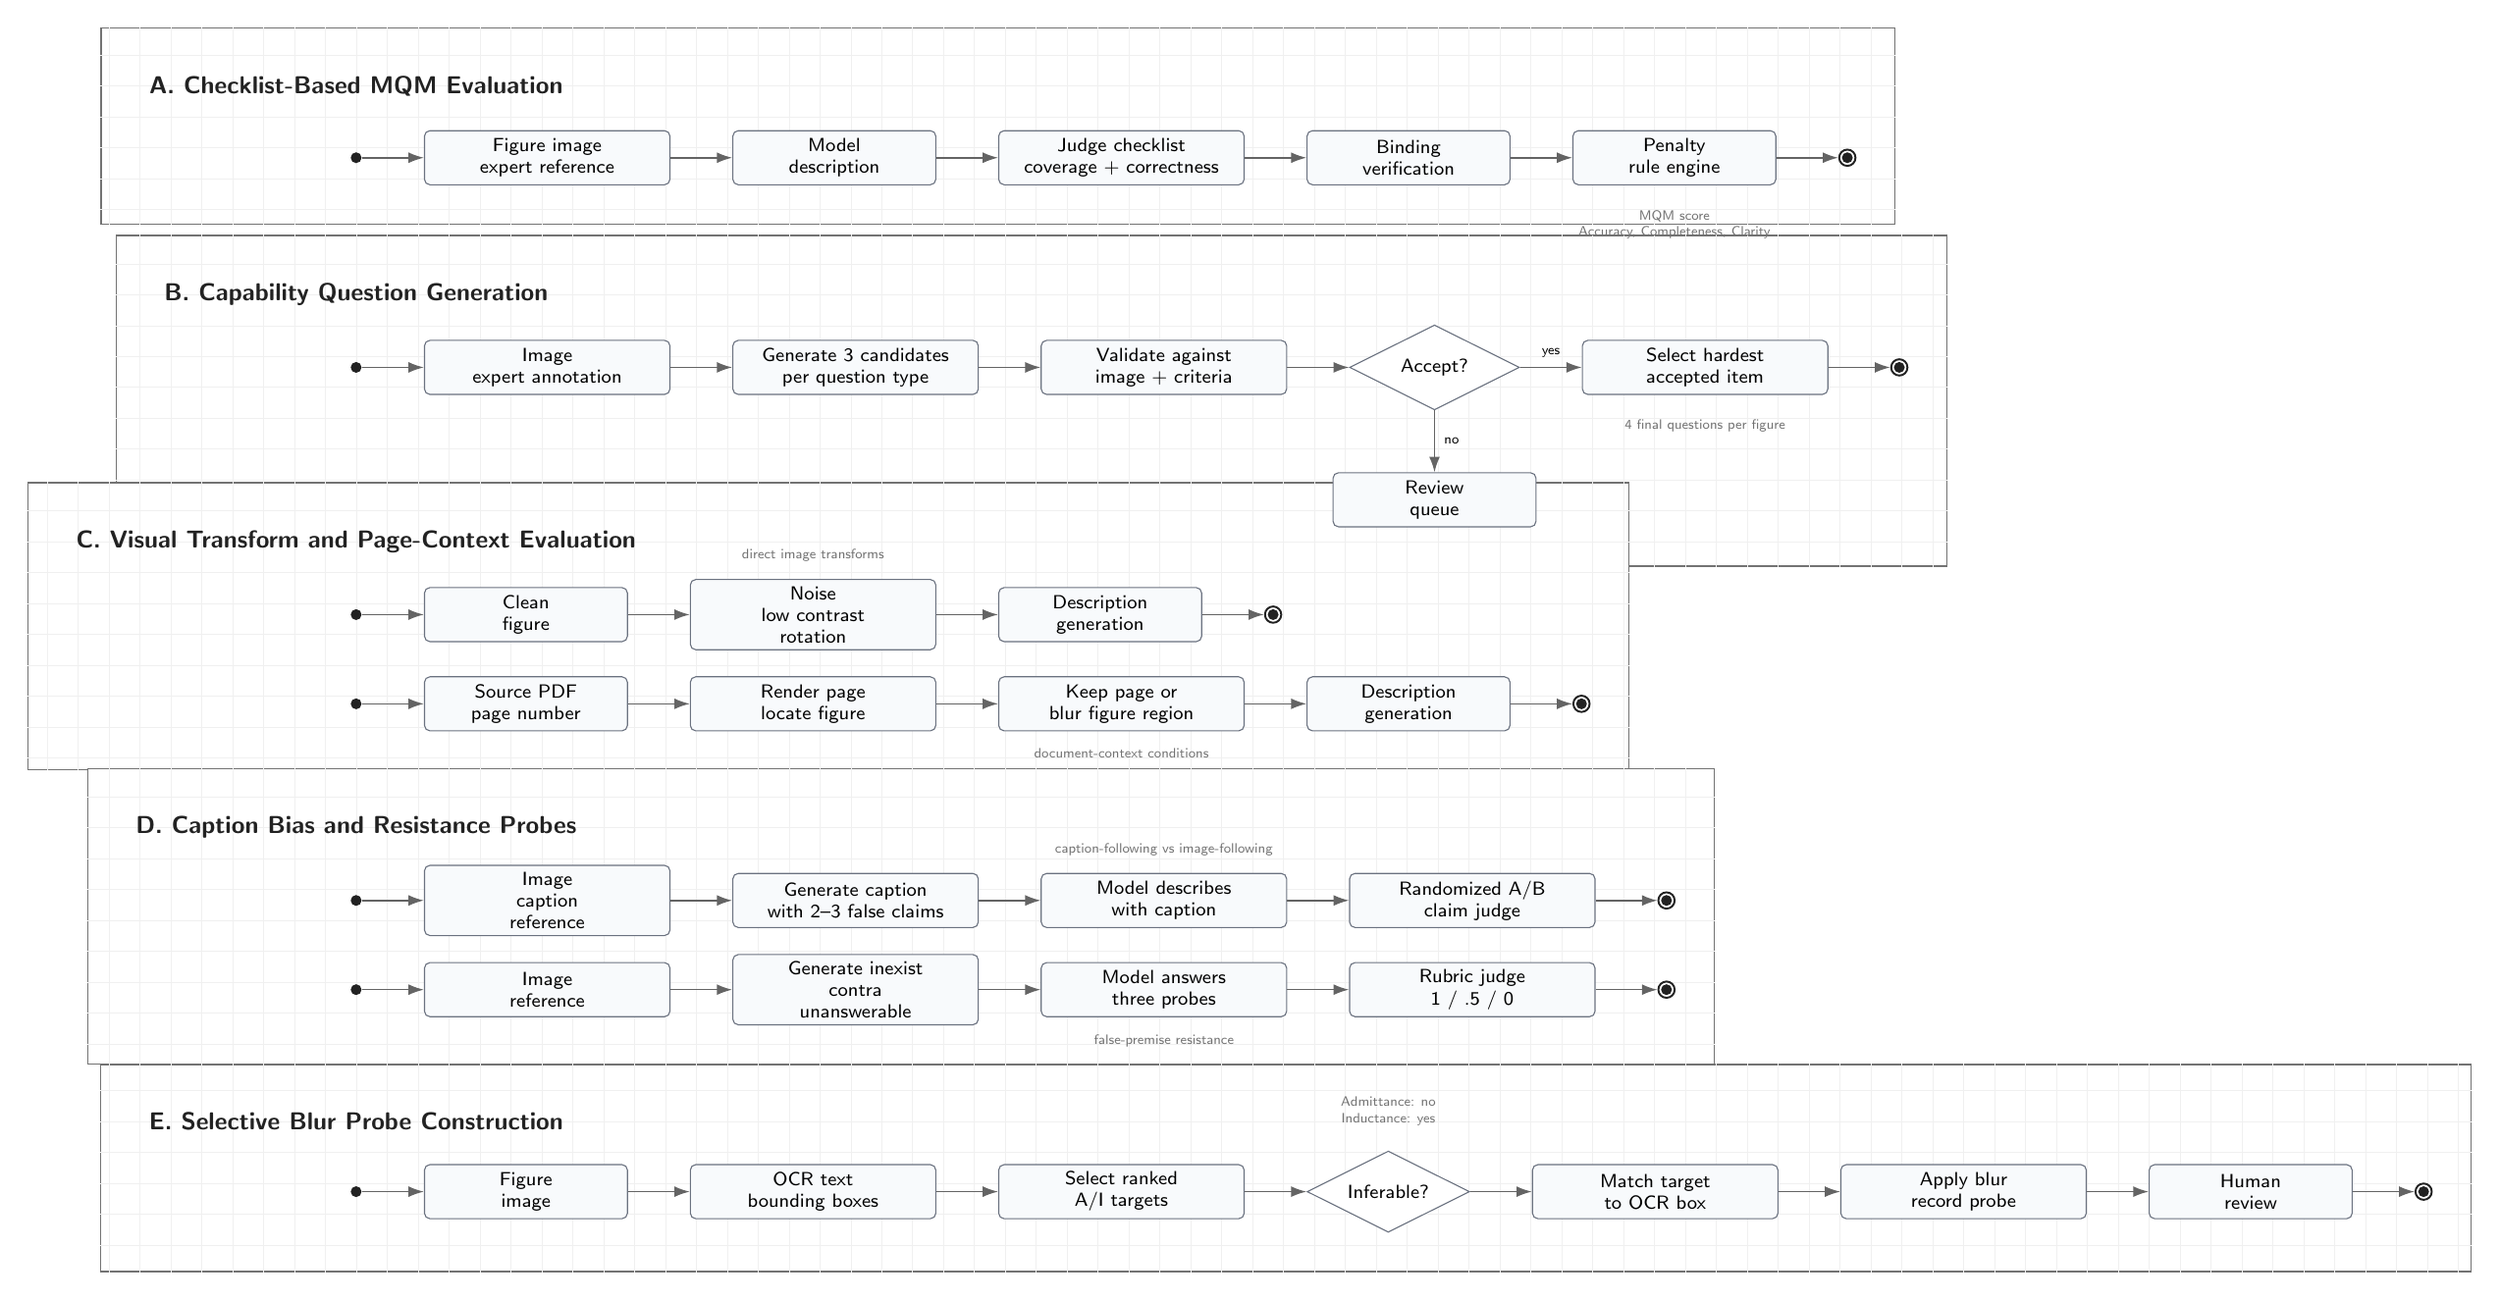
\begin{tikzpicture}[node distance=7mm and 8mm]

% MQM
\begin{scope}
\node[title] (mqmt) {A. Checklist-Based MQM Evaluation};
\node[start, below=6mm of mqmt] (s1) {};
\node[activitywide, right=of s1] (m1) {Figure image\\expert reference};
\node[activity, right=of m1] (m2) {Model\\description};
\node[activitywide, right=of m2] (m3) {Judge checklist\\coverage + correctness};
\node[activity, right=of m3] (m4) {Binding\\verification};
\node[activity, right=of m4] (m5) {Penalty\\rule engine};
\node[stop, right=of m5] (e1) {};
\draw[flow] (s1) -- (m1);
\draw[flow] (m1) -- (m2);
\draw[flow] (m2) -- (m3);
\draw[flow] (m3) -- (m4);
\draw[flow] (m4) -- (m5);
\draw[flow] (m5) -- (e1);
\node[note, below=2mm of m5] {MQM score\\Accuracy, Completeness, Clarity};
\panelgrid{(mqmt)(s1)(m1)(m2)(m3)(m4)(m5)(e1)}{mqm}
\end{scope}

% Capability
\begin{scope}[yshift=-2.7cm]
\node[title] (capt) {B. Capability Question Generation};
\node[start, below=6mm of capt] (s2) {};
\node[activitywide, right=of s2] (c1) {Image\\expert annotation};
\node[activitywide, right=of c1] (c2) {Generate 3 candidates\\per question type};
\node[activitywide, right=of c2] (c3) {Validate against\\image + criteria};
\node[decision, right=of c3] (c4) {Accept?};
\node[activitywide, right=of c4] (c5) {Select hardest\\accepted item};
\node[stop, right=of c5] (e2) {};
\node[activity, below=8mm of c4] (c6) {Review\\queue};
\draw[flow] (s2) -- (c1);
\draw[flow] (c1) -- (c2);
\draw[flow] (c2) -- (c3);
\draw[flow] (c3) -- (c4);
\draw[flow] (c4) -- node[above,font=\tiny]{yes} (c5);
\draw[flow] (c5) -- (e2);
\draw[flow] (c4) -- node[right,font=\tiny]{no} (c6);
\node[note, below=2mm of c5] {4 final questions per figure};
\panelgrid{(capt)(s2)(c1)(c2)(c3)(c4)(c5)(c6)(e2)}{cap}
\end{scope}

% Transforms
\begin{scope}[yshift=-5.9cm]
\node[title] (trt) {C. Visual Transform and Page-Context Evaluation};
\node[start, below=6mm of trt] (s3a) {};
\node[activity, right=of s3a] (t1) {Clean\\figure};
\node[activitywide, right=of t1] (t2) {Noise\\low contrast\\rotation};
\node[activity, right=of t2] (t3) {Description\\generation};
\node[stop, right=of t3] (e3a) {};
\node[start, below=10mm of s3a] (s3b) {};
\node[activity, right=of s3b] (t4) {Source PDF\\page number};
\node[activitywide, right=of t4] (t5) {Render page\\locate figure};
\node[activitywide, right=of t5] (t6) {Keep page or\\blur figure region};
\node[activity, right=of t6] (t7) {Description\\generation};
\node[stop, right=of t7] (e3b) {};
\draw[flow] (s3a) -- (t1);
\draw[flow] (t1) -- (t2);
\draw[flow] (t2) -- (t3);
\draw[flow] (t3) -- (e3a);
\draw[flow] (s3b) -- (t4);
\draw[flow] (t4) -- (t5);
\draw[flow] (t5) -- (t6);
\draw[flow] (t6) -- (t7);
\draw[flow] (t7) -- (e3b);
\node[note, above=1mm of t2] {direct image transforms};
\node[note, below=1mm of t6] {document-context conditions};
\panelgrid{(trt)(s3a)(t1)(t2)(t3)(e3a)(s3b)(t4)(t5)(t6)(t7)(e3b)}{tr}
\end{scope}

% Resistance / caption bias
\begin{scope}[yshift=-9.6cm]
\node[title] (rest) {D. Caption Bias and Resistance Probes};
\node[start, below=6mm of rest] (s4a) {};
\node[activitywide, right=of s4a] (r1) {Image\\caption\\reference};
\node[activitywide, right=of r1] (r2) {Generate caption\\with 2--3 false claims};
\node[activitywide, right=of r2] (r3) {Model describes\\with caption};
\node[activitywide, right=of r3] (r4) {Randomized A/B\\claim judge};
\node[stop, right=of r4] (e4a) {};
\node[start, below=10mm of s4a] (s4b) {};
\node[activitywide, right=of s4b] (r5) {Image\\reference};
\node[activitywide, right=of r5] (r6) {Generate inexist\\contra\\unanswerable};
\node[activitywide, right=of r6] (r7) {Model answers\\three probes};
\node[activitywide, right=of r7] (r8) {Rubric judge\\1 / .5 / 0};
\node[stop, right=of r8] (e4b) {};
\draw[flow] (s4a) -- (r1);
\draw[flow] (r1) -- (r2);
\draw[flow] (r2) -- (r3);
\draw[flow] (r3) -- (r4);
\draw[flow] (r4) -- (e4a);
\draw[flow] (s4b) -- (r5);
\draw[flow] (r5) -- (r6);
\draw[flow] (r6) -- (r7);
\draw[flow] (r7) -- (r8);
\draw[flow] (r8) -- (e4b);
\node[note, above=1mm of r3] {caption-following vs image-following};
\node[note, below=1mm of r7] {false-premise resistance};
\panelgrid{(rest)(s4a)(r1)(r2)(r3)(r4)(e4a)(s4b)(r5)(r6)(r7)(r8)(e4b)}{res}
\end{scope}

% Blur
\begin{scope}[yshift=-13.4cm]
\node[title] (blt) {E. Selective Blur Probe Construction};
\node[start, below=6mm of blt] (s5) {};
\node[activity, right=of s5] (b1) {Figure\\image};
\node[activitywide, right=of b1] (b2) {OCR text\\bounding boxes};
\node[activitywide, right=of b2] (b3) {Select ranked\\A/I targets};
\node[decision, right=of b3] (b4) {Inferable?};
\node[activitywide, right=of b4] (b5) {Match target\\to OCR box};
\node[activitywide, right=of b5] (b6) {Apply blur\\record probe};
\node[activity, right=of b6] (b7) {Human\\review};
\node[stop, right=of b7] (e5) {};
\node[note, above=2mm of b4] {Admittance: no\\Inductance: yes};
\draw[flow] (s5) -- (b1);
\draw[flow] (b1) -- (b2);
\draw[flow] (b2) -- (b3);
\draw[flow] (b3) -- (b4);
\draw[flow] (b4) -- (b5);
\draw[flow] (b5) -- (b6);
\draw[flow] (b6) -- (b7);
\draw[flow] (b7) -- (e5);
\panelgrid{(blt)(s5)(b1)(b2)(b3)(b4)(b5)(b6)(b7)(e5)}{blr}
\end{scope}

\end{tikzpicture}
\end{document}
